\paragraph{Gestione iscrizioni ad un questionario}
\label{Gestione iscrizioni ad un questionario}

\begin{figure}[ht]
	\centering
	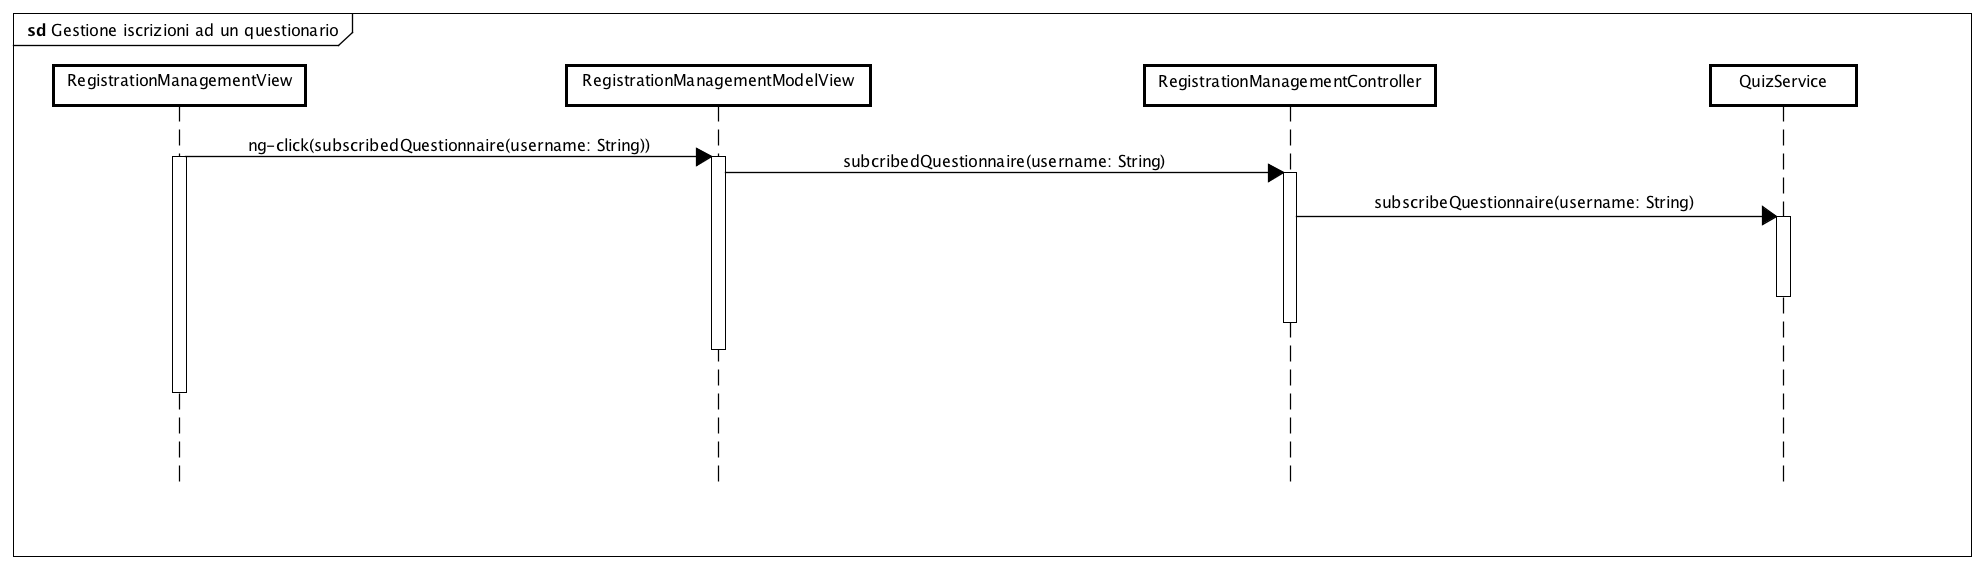
\includegraphics[scale=0.25,keepaspectratio]{UML/DiagrammiDiSequenza/Front-end/SubscriptionManagement.png}
	\caption{Recupero risultati del questionario}
\end{figure} \FloatBarrier
 
Al momento del dell'utente per confermare un iscrizione viene richiamato il metodo del \texttt{controller\ped{G}} che, a sua volta, richiama il metodo del \texttt{service\ped{G}} per eseguire la richiesta al back-end. Se la promessa ritornata dal \texttt{service\ped{G}} viene accettata allora verrà effettuata l'approvazione, altrimenti verrà restituito un oggetto contenente l'errore.
